\section{Work Process}
\label{WorkProcess}
The report and the product described in this report is created over the course of 12 weeks. We will be adapting on agile developing methods where we will work in iterations of 3 weeks. Once the iteration is planned we will not change it before we reach the end of the iteration, similar to extreme programming (XP), and in the beginning of each iteration adjust the schedule accordingly to the progress if needed, and have a supervisor meeting which will be our equivalent to a planning meeting. Unlike XP we will not have a dedicated on side customer other than our self, as this project will not be created with a customer in mind. We will be using a kanban like developing method, combined with a few ideas from XP as we have mentioned already. To use kanban we will use a kanbanflow/kanbanboard as our main scheduling and time tracking system, as we have used this with big success before for other projects. Kanban is also easily adaptable for smaller project, but we also want to use this as it can be used in a explorational way when working with new and unknown topics. Our plan is built up in iterations, but to use some of kanbans rules, the schedule may change over time to optimize and get the most out of our work time. The initial schedule can be seen in \figref{fig:InitTimeplan} and we will look at what changes that have occurred in section \ref{ProjectPlanning}.

The 12 weeks available for this project have been split into 4 iteration of 3 weeks which each have a theme. Iteration 1 is where the introduction, setup and planning will happen for the most, iteration 2 have focus on technologies we will be using, iteration 3 will be where the product mainly will come together and be optimized slightly, and the last iteration, iteration 4, will consist of conclusions and finalization of the last important parts that needs tweaking.


\begin{figure}[H]
	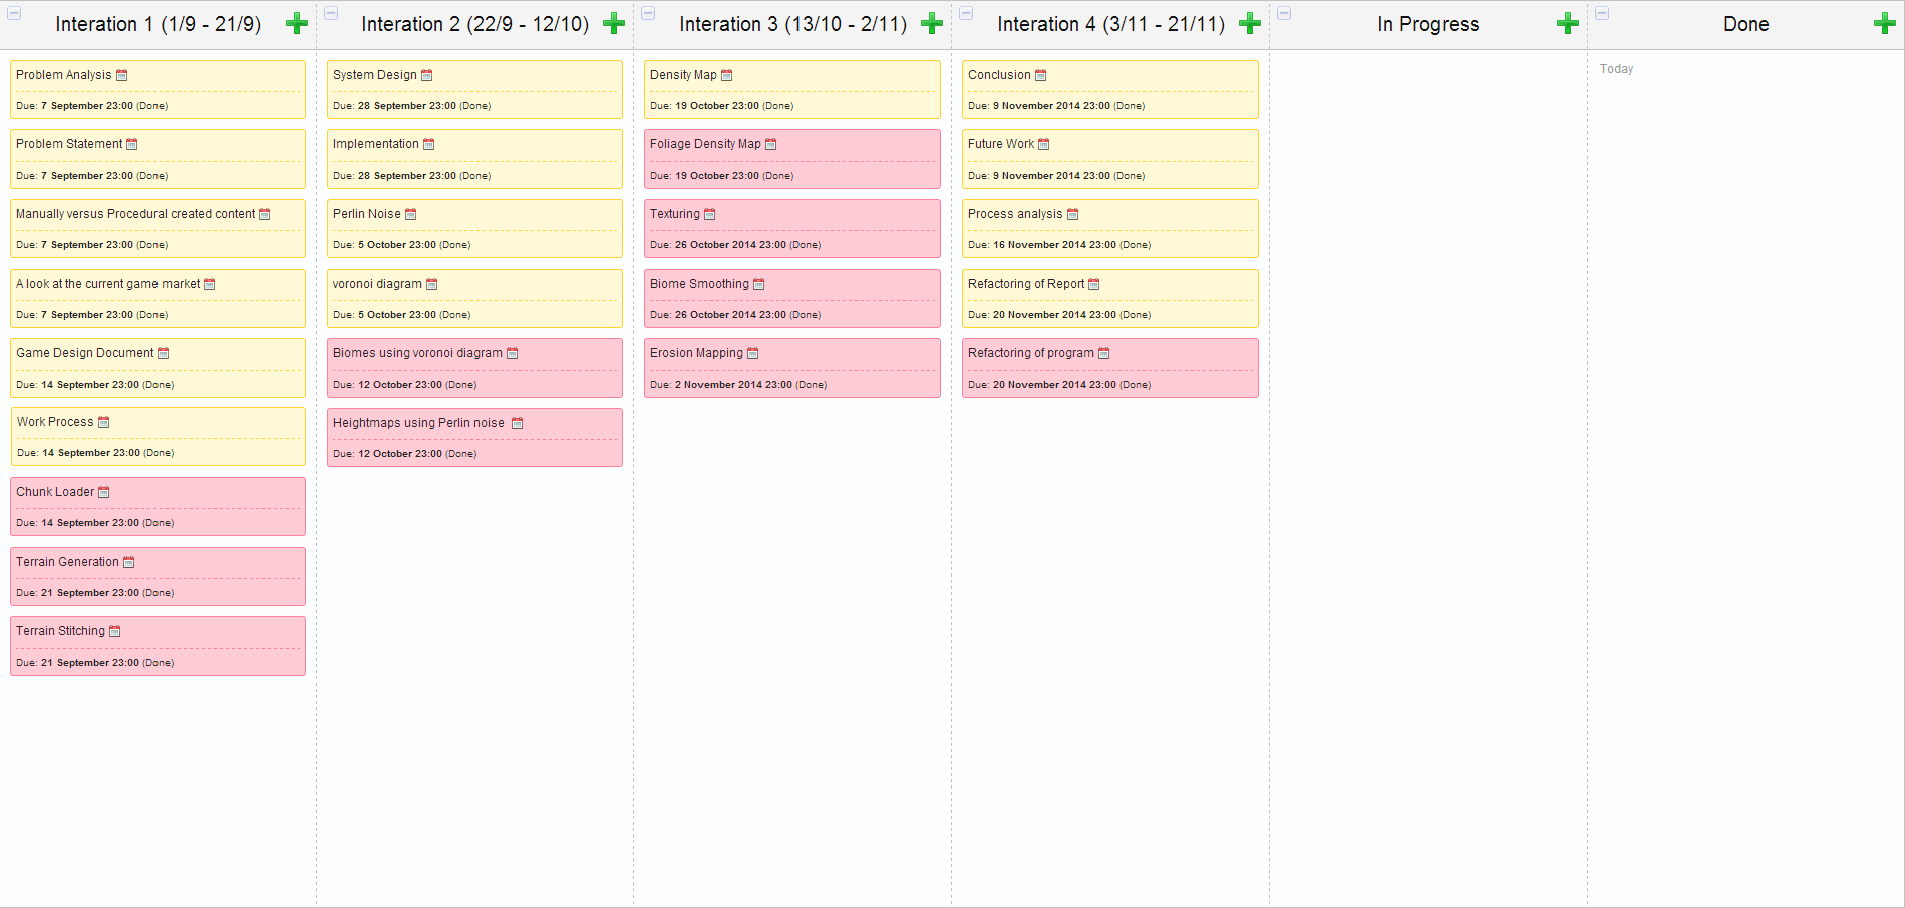
\includegraphics[width=1\linewidth]{img/InitTimeplan}
	\centering
	\caption{The initial time plan created for this project, the yellow blocks means the work is report related, where the red blocks are product related.}
	\label{fig:InitTimeplan}
\end{figure}
